\epart{Safety engineering}

\question{13}

In the projects in this subject, we have studied \emph{implantable cardioverter-defibrillators} (ICDs). This question is based on the same domain.

For this, assume that we have the ICD as specified in assignment 1, \emph{except} that there are three redundant heart-rate monitors operating in parallel, to mitigate the problem of faulty heart-rate monitors. In this system, the heart-rate monitors each provide a single reading to the ICD component, which uses approximate agreement majority voting to calculate a value for the heart rate.

Figure~\ref{fig:icd-loop} show ICD system architecture. Note the three heart rate monitors.

\begin{figure}[!h]
\centering
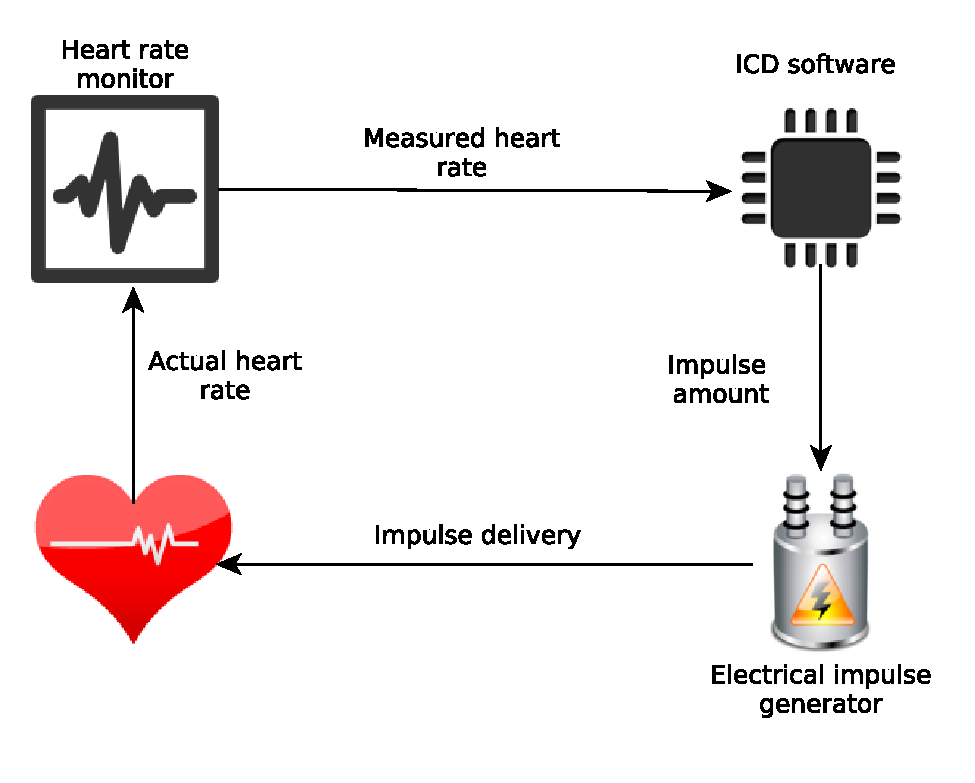
\includegraphics[scale=0.6]{./figs/icd-loop}
\caption{A model of the ICD system architecture.}
\label{fig:icd-loop}
\end{figure}


\subsubsection*{Safety conditions}

The following safety condition must be met by the ICD system:

\begin{quote}

 If the patient's heart is beating in a regular manner, they shall receive no shocks from the impulse generator.

\end{quote}

If this safety concern is violated, a hazard occurs.

Perform a fault tree analysis on the ICD software component for this hazard for the case when the heart receives a 30 joule shock. Your fault tree should outlines how the failure can occur, caused by the ICD software only. Briefly justify each choice that you make in your analysis, stating why you believe each level is \emph{necessary} or \emph{sufficient}.

The top-level event for the fault tree is the case in which the heart is shocked at 30 joules while having a regular heartbeat.

For this question, assume that the ICD software has the following functions:

 \begin{itemize}
  \item Receive the three heart rate readings (assume that heart rate monitors are functioning correctly).
  \item Vote on the three readings using an approximate agreement majority voting algorithm.
  \item Calculate the heart status: fibrillation, tachycardia, or normal. Fibrillation is when the standard deviation of the five previous readings is above a certain threshold.
  \item Calculate the joules to deliver.
  \item Send the intended amount of joules to the impulse generator (assume that impulse generator is functioning correctly).
 \end{itemize}



Figure~\ref{fig:safety:fault-tree-symbols} shows the syntax for fault trees, which you should use in your answer. 

%Marking: Should include the *normal case* that the heart beat is regular

\begin{figure}[!h]
  \centering

\vspace{10mm}

  \includegraphics[scale=0.79]{./figs/fault-tree-symbols}  \includegraphics[scale=0.6]{./figs/fault-tree-gates}
  \caption{Fault tree symbols}
  \label{fig:safety:fault-tree-symbols}
\end{figure}



\epart{Model-based specification}

\question{12}

Consider a messaging module of a system that maintains incoming and outgoing messaging queues for each process, and can send/receive messages from these queues.

The following Sum specification models the data types and state of the system. Total functions are used to model the message queue for each process.

\begin{verbatim}
  Bit == {0,1};
  Msg == seq Bit;

  [ProcessID];

  schema state is
  dec
    incoming : ProcessID --> seq Msg;
    outgoing : ProcessID --> seq Msg
  end state;
\end{verbatim}

To get the incoming message queue for a process, \verb+p+, we can use the expression \verb+incoming(p)+. 

For this question, the following Sum functions may be useful:

\begin{itemize}
  \item \verb+head(s)+: returns the first element in the sequence \verb+s+. For example, \verb+head(<3,2,1>)+ is equal to \verb+3+.
  \item \verb+tail(s)+: returns a sequence containing all but the first element in the sequence \verb+s+. For example, \verb+tail(<3,2,1>)+ is equal to \verb+<2,1>+.
  \item \verb+restrict(s, e)+: where \verb+s+ is a sequence and \verb+e+. Returns the sub-sequence of \verb+s+ containing only those elements in \verb+e+. For example, \verb+restrict(<4,3,2,1>, {5,3,1})+ is equal to \verb+<3,1>+.
\end{itemize}

\begin{enumerate}[(a)]
  
\item \textbf{[6 marks]} Model the following two operations: 

 \begin{itemize}
   \item \verb+Receive+, which takes as input, a message and a process ID, and adds the message to the incoming queue of the process ID.
   \item \verb+Send+, which takes as input, a process ID, and outputs the first message in the outgoing queue of that process, and removes the message from the queue.
 \end{itemize}

%The Receive operation must check that the queue is non-empty and report an error (or something similar)

\item \textbf{[6 marks]} Model the following operation:

\begin{itemize}
  \item \verb+ProcessIncoming+, which takes as input, a process ID, and then  outputs the first message in the \emph{incoming queue} of that process and removes that message from the queue, if and only if the party bit is correct. If not, an error is returned.

 This assumes that 1-bit parity coding is used for each message. That is, a single bit is added to added to the \emph{start} of the message (recall that the message is a sequence of bits):  0 if there are an odd number of 1s, and 1 if there are an even number of 1s. To process a received message from the incoming queue, the operation shall first check that the parity bit is correct.

\end{itemize}

\end{enumerate}

You do not need to get the syntax 100\% to obtain full marks for this question.

\epart{Fault-tolerant design}

\question{7}

N-version programming uses N different implementations to achieve fault tolerance. Consider two design scenarios: one in which N=2, and one in which N=3 (that is, a pair of redundant components, and a triple of redundant components).

Compare the 2-version programming and 3-version programming from the following points of view: 

\begin{enumerate}

 \item fault detection: that is, their ability to detect faults;

 \item fault tolerance: that is, their ability to tolerate faults;

 \item types of voting systems that could be used.

\end{enumerate}


\question{6}

Interlaces parity-bit coding can tolerate \emph{and detect} a 1-bit error in a string of bits by storing $N/2$ extra bits (where $N$ is the length of the information bits). The table for determining which bit is in error for an 8-bit information string is below.

\begin{center}
\begin{tabular}{lcccc}
 \toprule
     & \multicolumn{4}{l}{\textbf{Error in parity bit}}\\
     \cmidrule{2-5}
 \textbf{Bit error} & \textbf{P3} & \textbf{P2} & \textbf{P1} & \textbf{P0}\\
 \midrule
  $w_0$ & $\times$ & $\times$ & $\times$ & $\times$\\
  $w_1$ & $\times$ & $\times$ & $\times$ &         \\
  $w_2$ & $\times$ & $\times$ &          & $\times$\\
  $w_3$ & $\times$ &          & $\times$ & $\times$\\
  $w_4$ & $\times$ & $\times$ &          &         \\
  $w_5$ &          & $\times$ & $\times$ &         \\
  $w_6$ &          &          & $\times$ & $\times$\\
  $w_7$ &          & $\times$ &          & $\times$\\
  $P_0$ &          &          &          & $\times$\\
  $P_1$ &          &          & $\times$ &         \\
  $P_2$ &          & $\times$ &          &         \\
  $P_3$ & $\times$ &          &          &         \\
 \bottomrule
\end{tabular}
\end{center}

Assume a system in which a parity bit is 0 if there are an odd number of 1s, and 1 if there are an even number of 1s.

If a process receives the following 12-bits, with the first 8 containing the information and the remaining 4 containing the parity bits:
\begin{center}
   11111000-0110
\end{center}
Is any of the bits in this string in error? If so, which one? (Assume that at most 1 bit can be corrupted). Show your working.

%Solution: parity bit 3 is corrupt. The correct 4-bit parity code should be 0100.

\epart{Correctness by construction}

\question{1}

Who is the programming language \emph{Ada} named after, and why is this person famous?

\question{11}


Figure~\ref{fig:listave} shows an Ada program for calculating the average of an array of integers, and then overwrites the first element of the array with the value of the average. The program includes a contract with the postcondition:

\noindent \verb+Result = summation(1, List~'Length, List~)/List~'Length and List(1) = Result;+

where   {\tt summation(A,B,L) = $\sum_{i=A}^{B}$ \tt L($i$)}.

The program loops through all elements in the array, keeping a running tally in the variable {\tt Sum}. The loop invariant has been given in the assertion. At the end of the loop, the total sum is divided by the list length to give the average, unless the list is empty, in which case the result is 0. Finally, it puts the average value in the first element of the list.

Using Hoare logic, show that this program either establishes its contract, or fails to establish its contract. The Hoare logic rules are given in Figure~\ref{fig:hoare-logic}.

\begin{figure}[!h]
\begin{verbatim}
  type FloatArray is array(<>) of Float;

  procedure ListAverage(List : in FloatArray; Result : out Float)
  --# derives Result from List & List from List;
  --# post Result = summation(1, List~'Length, List~) / List~'Length
  --#      and List(1) = Result;
  is
    I, N : Integer;
    Sum : Float;
  begin
    Sum := 0.0;
    I := 1;
    N := List'Length;

    while I /= N loop
      --# assert Sum = summation(1, I, List);
      I := I + 1;
      Sum := Sum + List(I);
    end loop;

    if N = 0 then
      Result := 0.0;
    else
      Result := Sum / N;
    end if;

    List(1) := Result;

  end ListAverage;
\end{verbatim}

where {\tt summation(A,B,L) = $\sum_{i=A}^{B}$ \tt L($i$)}.

\caption{An Ada program for calculating the average from an array of integers.}
\label{fig:listave}
\end{figure}


\begin{figure}[!h]
\centering
%\begin{boxedminipage}{10.6cm}
\fullwidthbox{
\begin{tabular}{ll}
\\[4mm]
  $\{P[E/x]\}~ x := E~ \{P\}$ & (assignment axiom)\\[10mm]
$\{P\}~ \textbf{skip}~ \{P\}$ & (empty statement axiom)\\[10mm]
 $\begin{array}{c}
   P' \implies P,~  Q \implies Q', ~\{P\} ~S~ \{Q\}\\
 \hline
 \{P'\} ~S~ \{Q'\}
 \end{array}$ & (consequent rule)\\[10mm]
 $\begin{array}{c}
  \{P\} ~S_1~ \{R\},~~ \{R\} ~S_2~ \{Q\} \\
 \hline
 \{P\} ~S_1; S_2~ \{Q\}
 \end{array}$ & (sequential composition rule)\\[10mm]
$\begin{array}{c}
  \{P \land B\} ~S_1~ \{Q\},~~ \{P \land \neg B\} ~S_2~ \{Q\} \\
 \hline
 \{P\}~ \textbf{if}~ B ~\textbf{then}~ S_1 ~ \textbf{else}~ S_2 ~ \textbf{endif}~\{Q\}
 \end{array}$ & (conditional rule)\\[10mm]
 $\begin{array}{c}
  \{P \land B\} ~S~~\{P\}  \\
 \hline
 \{P\}~ \textbf{while}~ B ~\textbf{do}~ S ~ \textbf{done}~\{\neg B \land P\}
 \end{array}$ & (iteration rule)\\[10mm]
 $\begin{array}{c}
  \{P\}~S~ \{Q\}\\
\overline{\{P  [E_1/v_1, E_n/v_n]\} ~p(E_1, \ldots, E_n)~ \{Q [E_1/v_1, \ldots, E_n/v_n]\}}
 \end{array}$ & (procedure call rule)\\[10mm]
 $\{P[a\{NE \rightarrow E\}/a]\}~a[NE] := E~ \{P\}$ & (array assignment rule)\\[10mm]
\end{tabular}
}
\caption{Rules for Hoare logic.}
\label{fig:hoare-logic}
\vspace{10mm}
\begin{center}
\emph{--- End of exam ---}
\end{center}
\end{figure}



% LocalWords:  PoNR schedulable ECU ECUs List'Length Hoare Login ICDs
% LocalWords:  username AccessFile endif cardioverter ICD patient's
% LocalWords:  ProcessIncoming lcccc
